%Revisado
\section{Fase 2: Impacto Fotométrico e Sinal Físico (QP2)}
\label{sec:impacto_fotometrico}

Nesta fase, o efeito das condições de captura física é isolado para responder à Questão de Pesquisa QP2. O objetivo é demonstrar que a otimização da temperatura de cor da iluminação atua como um catalisador de performance, independentemente da arquitetura utilizada.

A evolução do MCC através das diferentes fontes de luz (AB, AM, BR) é ilustrada na Figura \ref{fig:h2_lighting}. Observa-se um crescimento consistente na performance de praticamente todos os classificadores à medida que a iluminação é otimizada para a luz branca (\textit{Cool White} 6000K), culminando nos melhores resultados absolutos na versão \textbf{V10}. Este fenômeno sugere que a qualidade do sinal físico de entrada é um preditor de sucesso mais forte que o ajuste fino algorítmico isolado.

\begin{figure}[h!]
  \centering
  \caption{Impacto da Iluminação (QP2): Evolução do MCC para cada arquitetura conforme a fonte de luz é otimizada fisicamente (AB para AM para BR).}
  \label{fig:h2_lighting}
  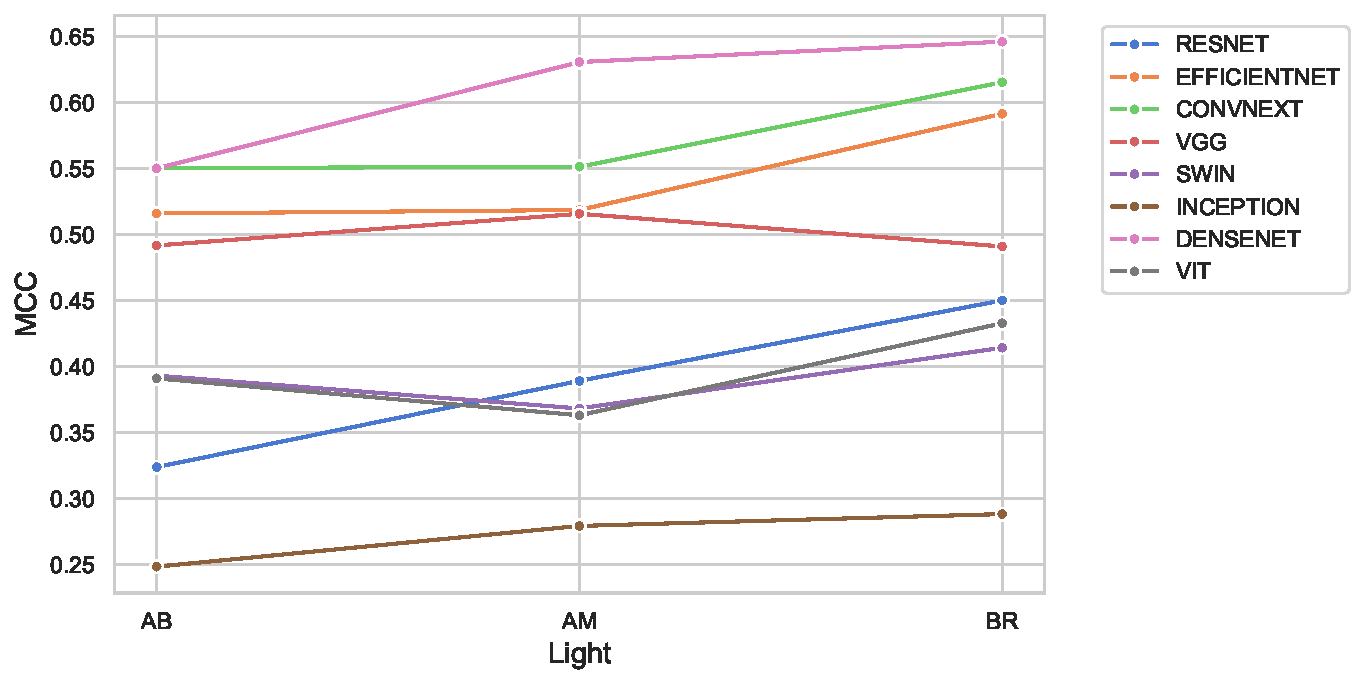
\includegraphics[width=0.8\textwidth]{images/h2_lighting_impact.pdf}
  \legend{Fonte: Do autor (2026).}
\end{figure}

Para conferir rigor estatístico a esta observação, redesenhou-se a análise usando cada \textbf{fardo físico de algodão} como bloco de medidas repetidas --- em vez das arquiteturas ---, isolando o efeito da luz da escolha do modelo. Para cada um dos $N=560$ fardos presentes nos três conjuntos de teste, calculou-se a probabilidade Softmax média atribuída pela ConvNeXt-Tiny (arquitetura de referência) à classe verdadeira, entre os patches daquele fardo disponíveis em cada condição de luz (em média, 1,8 patch por fardo por luz --- nem sempre os mesmos recortes exatos nas três condições, apenas do mesmo fardo). Aplicou-se o teste de \textbf{Friedman} sobre os postos resultantes: conforme apresentado na Tabela \ref{tab:friedman_detailed}, a luz \textbf{BR} obteve o maior posto médio ($2,26$), seguida por AM ($1,89$) e AB ($1,85$). O teste rejeita a hipótese nula $H_{0,2}$ ($\chi^2=59,19$, $p=1,41 \times 10^{-13}$), confirmando que a temperatura de cor da luz impacta significativamente a confiança/acurácia diagnóstica da rede.

\begin{table}[!h]
    \centering
    \begin{threeparttable}
    \caption{Teste de Friedman por fardo pareado: postos médios por condição de iluminação.}
    \label{tab:friedman_detailed}
    \begin{tabular}{lrc}
\toprule
\textbf{Versão do Dataset} & \textbf{Posto Médio} & \textbf{Grupo} \\
\midrule
V10 & 1.25 & (a) \\
V9 & 2.12 & (a) \\
V1 & 2.62 & (a) \\
V8 & 4.00 & (c) \\
\midrule
\multicolumn{3}{l}{\textbf{Estatística de Friedman}: $\chi^2 = 19.05$ ($p = 2.67e-04$)} \\
\multicolumn{3}{l}{\small Grupos com mesma letra não apresentam diferença estatística ($p > 0,05$)} \\
\bottomrule
\end{tabular}
    \begin{tablenotes}
            \small
            \item[] Fonte: Do autor (2026).
            \item[] Nota: Bloco = fardo físico ($N=560$); média de 1,8 patch por fardo por
            condição de luz (os patches podem diferir entre luzes --- ver texto).
        \end{tablenotes}
        \end{threeparttable}
\end{table}

A análise conjunta dos dados indica que a estabilização do cenário físico superou os ganhos obtidos pela simples troca de arquiteturas, reforçando a necessidade de ambientes controlados em aplicações de \textit{Edge AI} para o agronegócio.
